\section{The last board}\label{terminal}

\subsection{Geometry under the two laws}

When $K$ rows and $K$ columns are empty, the residual board is obtained from their $K^2$ empty
crossings by removing the unavailable ones, namely those that share a diagonal with a queen
already placed. Figure~\ref{fig:terminal} distinguishes the empty crossings from the \emph{mask},
the matrix $A=(Y_{ij})$ of their availability indicators.
\begin{figure}[htbp]
\centering
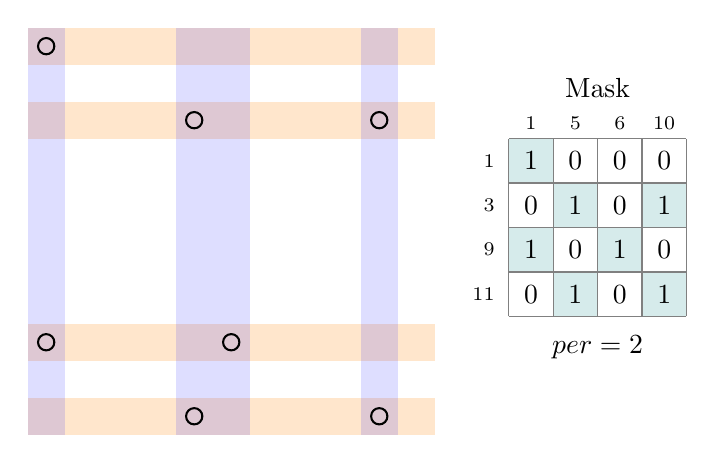
\begin{tikzpicture}[x=.47cm,y=.47cm]
 \bcuadricula{11}
 \foreach \rr in {1,3,9,11}{\fill[orange,opacity=.20] (0,{11-\rr}) rectangle (11,{12-\rr});}
 \foreach \cc in {1,5,6,10}{\fill[blue,opacity=.13] ({\cc-1},0) rectangle (\cc,11);}
 \foreach \rr/\cc in {1/1,3/5,3/10,9/1,9/6,11/5,11/10}{
  \bmarca{11}{\rr}{\cc}
  \draw[black,line width=.75pt] ({\cc-.5},{11.5-\rr}) circle[radius=.22];
 }
 \foreach \rr/\cc in {2/3,4/7,5/9,6/11,7/2,8/4,10/8}{\breina{11}{\rr}{\cc}}
 \begin{scope}[shift={(13,3.2)},scale=1.2]
  \node at (2,5.15) {Mask};
  \foreach \indice/\original in {1/1,2/5,3/6,4/10}
   {\node[font=\scriptsize] at ({\indice-.5},4.35) {$\original$};}
  \foreach \indice/\original in {1/1,2/3,3/9,4/11}
   {\node[font=\scriptsize,anchor=east] at (-.1,{4.5-\indice}) {$\original$};}
  \foreach \rr/\cc in {1/1,2/2,2/4,3/1,3/3,4/2,4/4}
   {\fill[teal!16] ({\cc-1},{4-\rr}) rectangle (\cc,{5-\rr});}
  \draw[step=1,gray,line width=.45pt] (0,0) grid (4,4);
  \foreach \rr/\valores in {1/{1,0,0,0},2/{0,1,0,1},3/{1,0,1,0},4/{0,1,0,1}}{
   \foreach \valor [count=\cc] in \valores
    {\node at ({\cc-.5},{4.5-\rr}) {$\valor$};}
  }
  \node at (2,-.7) {$\operatorname{per}=2$};
 \end{scope}
\end{tikzpicture}
\caption{Board of order eleven for the solution $\pi=(1,3,5,7,9,11,2,4,6,8,10)$ after removing
the queens in rows $1,3,9,11$. Rows are numbered from one, top to bottom, and columns from one, left
to right. Seven queens remain, shown as crowns. The bands highlight the four empty rows and the
empty columns $1,5,6,10$. The circled dots mark the available squares and correspond to the entries
equal to one in the mask, which retains the original labels. Row $1$ forces column $1$, and row $9$
then forces column $6$. Rows $3$ and $11$ can exchange $5$ and $10$, so the permanent is $2$. The positive
differences between rows are $2,6,8,10$, and those between columns are $1,4,5,9$. Since the two
sets are disjoint, no two empty crossings share a diagonal.}\label{fig:terminal}
\end{figure}


Recall that $F$ is the permanence event of Definition~\ref{def:regular}: the history reaches size
$K$, and all its boards, including the arrival board $B^{(K)}$, are regular. The figure illustrates the
geometry. In it, row 1 forces column 1, so every doubly stochastic matrix supported on the mask
assigns
zero mass to the available square $(9,1)$. The example lies outside $F$. Let $D_K$ be the event
that two distinct empty crossings of the board of size $K$ lie on the same diagonal of the initial
board. For $m\ge 1$, write $(u)_m=u(u-1)\cdots(u-m+1)$ if $u\ge m$, and $(u)_m=0$ if $0\le u<m$.

\begin{lema}[Shared diagonals on the last board]\label{terminal-geometria}
Under $\nu$ and under the law $\mu$ of a uniform solution revealed in an independent uniform order,
respectively, we have
\[
 \nu(F\cap D_K)\le d_{n,K}:=\frac{C K^4}{n}\,e^{C'/K},
 \qquad \mu(D_K\mid\pi)\le \frac{C K^4}{n}
\]
for every solution $\pi$. The second probability is taken over the order in which the rows
are revealed.
\end{lema}
\begin{proof}
The initial board has at most $Cn^3$ pairs of distinct squares sharing a diagonal. There are
$n^2$ choices for the first square and at most $2(n-1)$ choices for the second on its diagonals.
For both squares of a pair to be empty crossings at size $K$, two distinct rows and two distinct
columns must remain empty. On $F$ there was no earlier exit, so \eqref{prescr} with $s=t=2$
bounds the probability for each pair by $(K/n)^4e^{C'/K}$. A union bound gives the first claim.

For the second claim, fix $\pi$. The last $K$ rows in the uniform order form a uniform subset $I$
of size $K$. The corresponding columns are $\pi(I)$, and the empty crossings form $I\times\pi(I)$.
Figure~\ref{fig:testigos} shows how the row labels enter two such crossings.
\begin{figure}[htbp]
\centering
\begin{tikzpicture}[x=.53cm,y=.53cm]
 \foreach \tipo/\dx/\uno/\dos in {3/0/2/1,4/8.3/6/5}{
  \begin{scope}[shift={(\dx,0)}]
   \bcuadricula{6}
   \draw[red!75!black,line width=1.3pt] ({\uno-.5},5.5) -- ({\dos-.5},4.5);
   \bmarca{6}{1}{\uno}
   \bmarca{6}{2}{\dos}
   \draw[red!75!black,line width=1.2pt] ({\uno-.5},5.5) circle[radius=.45];
   \draw[red!75!black,line width=1.2pt] ({\dos-.5},4.5) circle[radius=.45];
   \foreach \rr/\cc in {1/2,2/4,3/6,4/1,5/3,6/5}{\breina{6}{\rr}{\cc}}
   \ifnum\tipo=3
    \node at (3,-1.1) {Three labels};
   \else
    \node at (3,-1.1) {Four labels};
   \fi
  \end{scope}
 }
\end{tikzpicture}
\caption{Two witnesses on the board of order six for the solution $\pi=(2,4,6,1,3,5)$. Rows
are numbered from one, top to bottom, and columns from one, left to right. The crowns are the
queens of $\pi$. Two circles joined by a line mark the squares $(i,\pi(j))$ and $(i',\pi(j'))$
that share a diagonal. On the left, $(i,i',j,j')=(1,2,1,4)$ marks $(1,2)$ and $(2,1)$ and uses
three distinct labels. On the right, $(1,2,3,6)$ marks $(1,6)$ and $(2,5)$ and uses four. With
only two labels we would have $\{i,i'\}=\{j,j'\}$ and $|i-i'|=|\pi(i)-\pi(i')|>0$, in which
case two queens of the solution would attack one another.}\label{fig:testigos}
\end{figure}


A pair sharing a diagonal has the form $(i,\pi(j)),(i',\pi(j'))$, with
\[
 |i-i'|=|\pi(j)-\pi(j')|>0,\qquad i,i',j,j'\in I.
\]
We call a quadruple of labels $(i,i',j,j')$ satisfying this equality of distances a \emph{witness},
whether or not its labels belong to $I$. Put $m=|\{i,i',j,j'\}|$. If $m=2$, the label pairs
$\{i,i'\}$ and $\{j,j'\}$ coincide. The equality of distances would imply that the queens of
$\pi$ in rows $i,i'$ attack each other, which is impossible. If $m=3$, fix $i,i'$ and specify
which of the two labels repeats and in which position $j,j'$ it occurs. The image of that label
under $\pi$ is known. The other image must be at distance $|i-i'|$ from it and hence has at most
two possible values. Each value determines its label via $\pi^{-1}$. Thus there are $O(n^2)$
three-label witnesses. For $m=4$, fixing $i,i',j$ leaves at most two possible values of $\pi(j')$,
giving $O(n^3)$ witnesses.

The subset $I$ contains $m$ fixed labels with probability $(K)_m/(n)_m\le(K/n)^m$ when $n\ge m$.
For $n\ge4$ a union bound gives
\[
 \mu(D_K\mid\pi)\le C\left[n^2(K/n)^3+n^3(K/n)^4\right]\le CK^4/n.
\]
Under $\mu$ the solution and the order can also be completed for histories that have already
stopped. Since $F\cap D_K\subseteq D_K$, integrating the estimate over $\pi$ also gives
$\mu(F\cap D_K)\le CK^4/n$.
\end{proof}
